\section{Problem Definition \& Methodology}
\label{sec:rerl}
We frame the problem of run time enforcement as a sequential decision making (SDM) one, by which the BIP engine has to be guided to select the set of interactions over an extended execution traces that maximize a cumulative return.  We formalize SDMs as the following five-tuple $\left \langle Q, \tilde{Q},\Gamma, \rightarrow, {R}_{+}, {R}_{-}, \gamma \right\rangle$.  Here, $Q$ represents the set of all possible states, $\tilde{Q} \subseteq Q$ the set of ``bad'' states that need to be avoided, $\Gamma$ the set of allowed interactions, and $\rightarrow$ represents the transition model. $R_{+}$ and ${R}_{-}$ are two positive and negative scalar parameters, which allow us to define the reward function quantifying the selection of the engine.
Clearly, the engine gets rewarded when in a state $ \bm{q} \notin \tilde{Q}$, while penalized if $ \bm{q} \in \tilde{Q}$. Using this intuition, one can define a reward function of the states written as: 


\begin{displaymath}
   \mathcal{R}( \bm{q}) = \left\{
     \begin{array}{lr}
       R_{+} & :   \bm{q} \notin \tilde{Q} \\
       R_{-} & :  \bm{q} \in \tilde{Q}.
     \end{array}
   \right.
\end{displaymath} 
Given the above reward definition, we finally introduce $\gamma \in [0,1)$ to denote the discount factor specifying the degree to which rewards are discounted over time as the engine interacts with each of the components. 

At each time step $t$, the engine observes a state $ \bm{q_{t}} \in Q$ and must choose an interaction $a_{t} \in \mathcal{A}_{ \bm{q_t}} \subseteq \Gamma$, transitioning it to a new state $ \bm{q_{t}} \goesto[a_{t}] \bm{q_{t+1}}$ as given by $\rightarrow$ and yielding a reward $\mathcal{R}\left( \bm{q_{t+1}}\right)$, where $\mathcal{A}_{q_t}$ denotes all enabled interactions from state  $q_{t}$, i.e., $\mathcal{A}_{ \bm{q_t}} = \{a \mid \exists  \bm{q'}:  \bm{q_{t}} \goesto[a]  \bm{q'} \in \rightarrow\}$. 
We filter the choice of the allowed interactions, i.e., $\mathcal{A}_{ \bm{q_t}}$, at each time-step by an interaction-selection rule, which we refer to as the policy $\pi$. We extend the sequential decision making literature by defining policies that map between the set of states, $Q$, and any combination of the allowed interactions, i.e., $\pi: Q \rightarrow 2^{\Gamma}$, where for all $ \bm{q} \in Q: \pi( \bm{q}) \subseteq\mathcal{A}_{ \bm{q}}$.
Consequently, the new behavior of the composite component, guided by the policy $\pi$, is defined by $C_\pi = (Q, \Gamma, \goesto_\pi)$, where $\goesto_\pi$ is the least set of transitions satisfying the following rule:
\begin{mathpar}
\inferrule*
	{
       \bm{q} \goesto[a]  \bm{q'} \and
      a \in \pi( \bm{q})
    }
    {
       \bm{q} \goesto[a]_\pi  \bm{q'}
    }
\end{mathpar}

The goal now is to find an optimal policy $\pi^{\star}$ that maximizes the \emph{expected} total sum of the rewards it receives in the long run, while starting from an initial state $ \bm{q_{0}} \in Q$. We will evaluate the performance of a policy $\pi$ by:
\begin{equation}
\label{Eq:ValueOne}
\texttt{eval}({\pi}| \bm{q_{0}})  = \mathbb{E}_{\bm{\rho}(C_\pi)} \left[\sum_{t=0}^{T} \gamma^{t}\mathcal{R}( \bm{q_{t+1}})\right],
\end{equation}
where  $\mathbb{E}_{\bm{\rho}(C_\pi)}$ denotes the expectation under all the set of all the allowed (by the policy $\pi$) possible traces, and $T$ is the length of the trace. 


Notice that we index the value of the state by the policy $\pi$ to explicitly reflect the dependency of the value on the policy being followed from a state $ \bm{q_{t}}$. Interestingly, the definition of the evaluator asserts that the value of a state $ \bm{q_{t}}$ is the expected instantaneous reward plus the expected discounted value of the next state. Clearly, we are interested in determining the optimal policy $\pi^{\star}$, which upon its usage yields maximized values for any $ \bm{q_{t}} \in Q$. As such our goal is to determine a policy $\pi$ that solves:
\begin{equation*}
\pi^{\star} \equiv \max_{\pi} \texttt{eval}({\pi}| \bm{q_{0}}). 
\end{equation*}

%In other words, rather than targeting the determination of $\pi^{\star}$ directly, we will seek the \emph{value} of a state $q \in Q$. %Clearly, one can recover the current iteration policy $\pi$ using:
%$
%\pi(q) = \texttt{argmax}_{a}\{V(q') \mid q \goesto[a] q'\}
%$.


Finally, being in a state $ \bm{q}$, we quantify the performance of the state-interaction pairs using the function $\mathbb{P}: Q \times \Gamma \rightarrow \mathbb{R}$. Given such a performance measure $\mathbb{P}$, the engine can follow the policy $\pi$, defined as follows: 
\begin{equation}
\label{Eq:Policy}
\pi( \bm{q}) = \arg\max_{a} \{\mathbb{P}( \bm{q},a) \mid a \in {\cal A}( \bm{q})\}.
\end{equation}
In other words, given a state $ \bm{q}$, policy $\pi$ selects the enabled interaction that has maximum evaluation from that state. Clearly, an interaction must have a maximum evaluation when it is guaranteed that its execution will not lead to a bad state. 

In what comes next, we define two methods capable of computing such performance measures, i.e., $\mathbb{P}$,  (consequently policies) in finite as well as infinite state-space. 

\subsection{Finite State-Space - Value Iteration}
Due to the number of possible policies at each time step, it is a challenge to compute the value for all possible options. Instead, we propose the application of a dynamic programming algorithm known as value iteration, summarized in Algorithm~\ref{Algo:VI} to find the optimal policy efficiently. 
\begin{algorithm}[h!]
\caption{Value Iteration for Run Time Enforcement}
\label{Algo:VI}
\begin{algorithmic}[1]
\STATE \textbf{Input:} Initialization of $V( \bm{q})$ for all $ \bm{q}\in Q$, precision parameter $\epsilon$
\STATE $\mathtt{error = \epsilon + 1} $
\WHILE {$\mathtt{k} < \mathtt{bound} \, \wedge \, \mathtt{error} \geq \epsilon$}
	\FOR {\textbf{each} $ \bm{q} \in Q$ }
		\FOR {\textbf{each} $a \in \mathcal{A}_a$}
			\STATE $\mathtt{tmp} = \mathcal{R}( \bm{q^{\prime}}) + \gamma V( \bm{q^{\prime}})$, where $ \bm{q} \goesto[a] \bm{q^{\prime}}$
		\STATE $\mathtt{error} =\max(\mathtt{error}\, , \, |\mathtt{tmp} - \mathbb{P}( \bm{q}, a)|)$
			\STATE $\mathbb{P}( \bm{q}, a) = \mathtt{tmp}$
		\ENDFOR
	\STATE $V( \bm{q}) =  \max_{a \in {\cal A}} \mathbb{P}( \bm{q}, a)$
	\ENDFOR
	\STATE $\mathtt{k = k + 1}$
\ENDWHILE
\end{algorithmic}
\end{algorithm}

In essence, Algorithm~\ref{Algo:VI} is iteratively updating the performance measures of all the state-interaction pairs (until either (1) we reach a predefined bound, i.e., $\mathtt{bound}$; or (2) the values are within a predefined $\epsilon$),  by choosing these actions that maximize the instantaneous rewards, as well as the future information encoded through $V(q^{\prime})$. 
%Defining the operator $$\mathcal{T}^{\pi} = \max_{a} \left[\mathcal{R}(q) + \gamma \sum_{q \goesto[a]q^{\prime}}V_{k}(q^{\prime})\right],$$ one can easily see that the optimal value function is essentially  fixed-point of $V_{k+1} = \mathcal{T}^{\pi}  V_{k}$. 
Contrary to state-space-exploration algorithms, our method remedies the need to construct the full labeled transition system as we only require the knowledge of the successor state from a given state and action pair with no regard to its reachability properties. Furthermore, notice that though line~4 in Algorithm~\ref{Algo:VI} requires a loop over all states computational time can be highly reduced by following a sampling-based procedure, where fractions of the state-space are considered. Notice, however, the successfulness of the attained policy comes hand-in-hand with the fraction of the state space sampled. In other words, the higher the fraction, the closer to optimality is the policy and vice versa. 


\subsection{Infinite State-Space - Deep Value Iteration}
The methodology detailed so-far suffers when considering infinite state-spaces as it requires exact representation of performance measures and policies. In general, an exact representation can only be achieved by storing distinct estimates of the return for every state-interaction pair. When states are continuous, such exact representations are no longer possible and performance measures need to be represented approximately. 

Approximation in the continuous setting is not only a problem of representation. Two additional types of approximation are needed. Firstly, sample-based approximation is necessary in any of these frameworks. Secondly, the algorithm must repeatedly solve a difficult minimization problem. To clarify, consider Algorithm~\ref{Algo:VI}, where every iteration necessitates a loop over \emph{every state-interaction pair}. When state space contains an infinite number of elements, it is impossible to loop over all pairs in finite time. Instead, a sample-based update that only considers a finite number of such pairs has to be used. 

In this section, our goal is to develop an algorithm capable of avoiding the problems above. This ultimately leads us to a method for run-time enforcement operating in continuous state spaces. 
To commence, we introduce a function approximator, encoded through a neural network (NN), to represent a
good approximation of performance measures of all state-interaction pairs. The goal of this approximator is to \emph{autonomously generalize} over the state-space, such that similarly behaving states cluster together. Before commencing with our algorithm, we next introduce a concise introduction to NNs, accompanied with its generalization to the deep setting. 

\subsection{Neural Networks (NNs)}
In an artificial NN, a neuron is a logistic unit, which is fed inputs through input wires. This unit can perform computations resulting in outputs that are transmitted through the output wires. 
\begin{wrapfigure}{r}{7cm}
\vspace*{-0.6cm}
\label{Fig:FigTwo}
\centering 
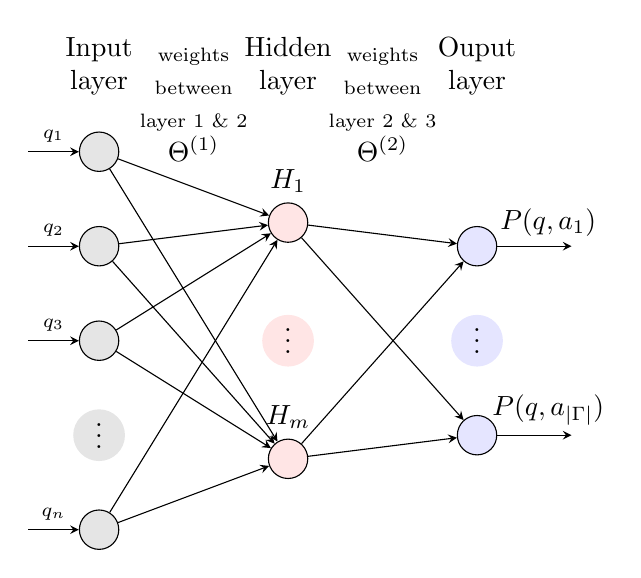
\begin{tikzpicture}[x=1.2cm, y=1.2cm, >=stealth]
\tikzset{%
  every neuron/.style={
    circle,
    draw,
    minimum size=0.5cm
  },
  neuron missing/.style={
    draw=none, 
    scale=1,
    text height=0.333cm,
    execute at begin node=\color{black}$\vdots$
  },
}

\foreach \m/\l [count=\y] in {1,2,3,missing,4}
  \node [fill=black!10,every neuron/.try, neuron \m/.try] (input-\m) at (0,2.5-\y) {};

\foreach \m [count=\y] in {1,missing,2}
  \node [fill=red!10,every neuron/.try, neuron \m/.try ] (hidden-\m) at (2,2-\y*1.25) {};

\foreach \m [count=\y] in {1,missing,2}
  \node [fill=blue!10,every neuron/.try, neuron \m/.try ] (output-\m) at (4,1.5-\y) {};

\foreach \l [count=\i] in {1,2,3,n}
  \draw [<-] (input-\i) -- ++(-0.75,0)
    node [above, midway] {\scriptsize$q_\l$};

\foreach \l [count=\i] in {1,m}
  \node [above] at (hidden-\i.north) {$H_\l$};

\foreach \l [count=\i] in {1,|\Gamma|}
  \draw [->] (output-\i) -- ++(1,0)
    node [above, midway] {\quad $\mathbb{P}(\bm{q}, a_{\l})$};

\foreach \i in {1,...,4}
  \foreach \j in {1,...,2}
    \draw [->] (input-\i) -- (hidden-\j);

\foreach \i in {1,...,2}
  \foreach \j in {1,...,2}
    \draw [->] (hidden-\i) -- (output-\j);

\foreach \l [count=\x from 0] in {Input, Hidden, Ouput}
  \node [align=center, above] at (\x*2,2) {\l \\ layer};
\node[align=center] at (1,2) {\scriptsize weights \\ \scriptsize between \\ \scriptsize layer 1 \& 2 \\ $\bm{\Theta}^{(1)}$};
\node[align=center] at (3,2) {\scriptsize weights \\ \scriptsize between \\ \scriptsize layer 2 \& 3 \\ $\bm{\Theta}^{(2)}$};
\end{tikzpicture}
\vspace*{-0.3cm}
\caption{A high-level depiction of an artificial NN.}
\vspace*{-0.3cm}
\end{wrapfigure}
An artificial NN is simply a set of these logistic units strung together as shown in Figure~\ref{Fig:FigTwo}. Each two layers are connected together using weight parameters. As such, the NN in Figure~\ref{Fig:FigTwo} possesses two weighting matrices, $\bm{\Theta}^{(1)}$ and $\bm{\Theta}^{(2)}$. Here, we used $\bm{\Theta}^{(l)}$ to denote the weights connecting layers $l$ and $l+1$. Definitely, the dimensionality of $\bm{\Theta}^{(l)}$ depends on the number of units in each of the two layers\footnote{
In practice, a bias term is added to increase the expressiveness of the functions learnt by the NN.}. 
%\vspace*{-0.4cm}
For example, in our case, the dimension of the input layer is equal to the number of components, and the dimension of the output layer is equal to number of interactions. The number of hidden layers and the number of neurons per hidden layer can be configured depending on the functions to be learnt. 
%For example, if layer $l$ consists of $s_{l}$ units and layer $l+1$ of $s_{l+1}$, $\bm{\Theta}^{(l)}$ has a dimensionality of $s_{l+1} \times s_{l} +1$, where we have added another dimension to incorporate the bias term (incorporated to increase the expressiveness of the functions learnt by the neural network). 
%

\paragraph{Feed Forward.}
Given the notation introduced above, we are now ready to discuss the computations that are performed by a NN. Intuitively, between every two layers the inputs from the previous layer are, first, linearly (through the weight matrices) propagated forward and then nonlinearly transformed (through the sigmoids) to produce an output on the successor layer. Recursing this process, which we refer to as forward propagation, over the total layers of the network will produce an output on the final layer $L$. 
%
\vspace*{-0.3cm}
\paragraph{Training \& Backward Propagation.} Having described feed forward propagation, the next step is to detail the strategy by which NNs determine the model parameters (i.e., the $\bm{\Theta}^{(l)}$ matrices -- denoted by $\bm{\Theta}$, i.e., $\bm{\Theta} = \{\bm{\Theta^{(1)}}, \dots, \bm{\Theta^{(l)}}\}$). In standard regression or classification problems, back-propagation is the algorithm adopted. Given an input data point, back-propagation commences as follows. First, forward propagation is executed and the network is made to output a value. This value is then compared to the real output from the data set producing an error. This error is then propagated backwards to every other layer and used to update connecting weights. Such updates typically involve gradient-based methods (e.g., stochastic gradients).  

Unfortunately, the direct application of NNs in our context is challenging since the performance measures $\mathbb{P}$ has to build, through sampling, a \emph{labeled} data set (with states being inputs and state-interaction values as outputs) to train on. The goal now is to determine at compile-time a good approximation of $\mathbb{P}$ through exploring an infinite state-space. 

\subsection{Deep Value Iteration -- Infinite State Space}
In Algorithm~\ref{Algo:VI2}, we present a solution for approximating the performance measures $\mathbb{P}_{\bm{\Theta}}$\footnote{Note that $\mathbb{P}$ is indexed by ${\bm{\Theta}}$ as its output depends on ${\bm{\Theta}}$.} of all the state-interaction pairs in case of infinite state-space.

In particular, we use an NN that takes a BIP state as input, encoded as a vector of size $n$, where $n$ is the number of atomic components (i.e., the $i^{\text{th}}$ input encodes the local state of atomic component $B_i$). The output of the NN encodes the performance measures $\mathbb{P}$ for each interaction. As such, the $i^{\text{th}}$ output of the NN encodes the safety of executing interaction $a_i$.  

On a high-level, the algorithm operates in two loops. The first is episode-based, while the second runs for a horizon $T$. At each episode, the goal is to collect relevant labeled data, encoding a trace of the system, to improve the approximation -- encoded through the NN -- of the performance measure, as summarized in lines 5-10 in the algorithm. 

A trace is selected as follows. First, the algorithm selects an allowed interaction either randomly with a probability $\epsilon$ (i.e., exploration) or by exploiting the current estimate of the performance measure. In other words, given the current state $ \bm{q}$, forward propagation is first executed to produce  $\mathbb{P}_{\bm{\Theta}}( \bm{q},a_i)$. As such, the enabled interaction that has a maximum performance measure is selected, i.e., $\arg\max_{a\in {\cal A}_q} \mathbb{P}_{\bm{\Theta}}( \bm{q},a)$. 
Next, the engine executes the interaction and stores both the dynamical transition and its usefulness (i.e., reward) in a replay memory data set, $\mathcal{D}$. 

To ensure that the learning algorithm takes learning memory into account, we sample a set of size $N_{2}$, with the help of alternative NN (with weight matrices $\bm{\Theta}^{-}$). This is due to the fact that the backward propagation (used for training) discussed previously operates successfully for relatively ``shallow'' networks, i.e., networks with low number of hidden layers. As the number of these layers increases (i.e., deep NN), propagating gradients backward becomes increasingly challenging leading to convergence to local minima. To circumvent the above problems, we adapt a solution by which gradient updates are not performed at each iteration of the training algorithm. In particular, we assume additional knowledge modelled via an alternative NN that encodes previously experienced traces. This NN is used as a reference that we update after a preset number of iterations. As such, old knowledge encountered by the agent is not hindered by novel observations. 

Consequently, we form a data set $\mathcal{D}$  (line~8)  in preparation to retrain the original NN, while taking the history of traces into account. The process by which we generate these labels is in essence similar to finite value iterator. The main difference, however, is the usage of sample-based transitions to train a NN.  
\begin{algorithm}[h!]
\caption{Deep-Value Iteration for Run Time Enforcement in Continuous States}
\label{Algo:VI2}
\begin{algorithmic}[1]
\STATE Initialize replay memory $\mathcal{D}$ to capacity $N$, and the NN weights randomly, $K$
\FOR {$\text{episode} = 1 \ \ \text{to} \ \ M$}
\STATE Set initial state to $ \bm{q_{0}}$
\FOR  {$t=1$ \ \ \text{to} \ \ T}
\STATE With some probability $\epsilon$ select a random interaction $a_{t}$
\STATE With a probability $1 - \epsilon$ select interaction $a_{t} = \arg\max_{a\in {\cal A}(q_t)}\mathbb{P}_{\bm{\Theta}}( \bm{q_t},a)$
\STATE Execute interaction $a_{t}$ and observe reward, $r_{t+1}$, and successor state $ \bm{q_{t+1}}$
\STATE Store transition $\left( \bm{q_{t}}, a_{t}, r_{t+1},  \bm{q_{t+1}}\right)$ on replay memory $\mathcal{D}$
\STATE Sample random minibatch of transitions $\left( \bm{q_{j}}, a_{j}, r_{j+1},  \bm{q_{j+1}}\right)$ of size $N_{2}$ from $\mathcal{D}$ and create output label by 
\begin{displaymath}
   y_{j} = \left\{
     \begin{array}{lr}
       r_{j+1} & \text{if $q_{j+1}$ is a bad state}\\
        r_{j+1} + \gamma \max_{a \in {\cal A}_{q_{j+1}}} \mathbb{P}_{\bm{\Theta^{-}}}(q_{j+1},a)  & \text{if $q_{j+1}$ is a correct state}
     \end{array}
   \right.
\end{displaymath} 
\ENDFOR
\STATE Retrain network on the $N_{2}$ data points with $y_{j}$ being the labels. 
\STATE Update ${\bm{\Theta^{-}}}$ to ${\bm{\Theta}}$ every $K$ episodes.
\ENDFOR
\end{algorithmic}
\end{algorithm}

%In other words, starting from randomly initialized weights, $\bm{\theta}$, the engine has to 1) gather relevant traces from the environment, and 2) improve its estimate of $\bm{\theta}$ to maximize its return. Having 

%The goal of such a neural net is to enable continuous states by autonomously generalizing similar...


\subsection{Fairness}
Deep value iteration allows to compute $\bm{\Theta}$, and hence $\mathbb{P}_{\bm{\Theta}}$ for all state-interaction pairs. As defined in Equation~\ref{Eq:Policy}, the policy then can be defined using $\mathbb{P}$. For this, as we are dealing with real numbers, the same trace would be selected all the time by engine, which is running that policy. As such, other correct traces will not be reachable in the obtained system. For instance, given a global state, a policy would select the interaction leading to a state with maximum performance measure value, even though there exist other interactions leading to other correct traces. To remedy this, we define a fair policy that is allowed to deviate from the optimal policy with a degree of fairness.  The fair policy is defined as follows. 
\begin{equation}
\label{Eq:Policy-fair}
\pi(\bm{q}) = \{a \mid q \goesto[a] q' \wedge \mathbb{P}_{\bm{\Theta}}(q, a) \geq \mathtt{max_q} - \mathtt{fair}\},
\end{equation}
where, $\mathtt{max_q} = \max_{a \in {\cal A}_q}\mathbb{P}_{\bm{\Theta}}(q, a)$.  $\mathtt{fair}$ is the tolerance against the optimal policy. The value of $\mathtt{fair}$ depends on (1) the value of good and bad rewards, and (2) the  horizon used in deep value iteration algorithm. Clearly, the more fairness the more deviation from the optimal policy we get. 